\section{Достоверность партонной модели при ПэВ-энергиях}
\label{sec:dis_reliability}
На рис. (\ref{fig:xQ2_PDG}) приведена исследованная область в экспериментах на коллайдерах:   БАК (LHC), Теватрон, HERA, а также в экспериментах с неподвижной мишенью. В области малых $x\lesssim 10^{-6}$ экспериментальные измерения практически отсутствуют. Между тем, с ростом энергии взаимодействия нейтрино, вклад именно малых $x$ в сечение взаимодействия становится доминирующим. Выход в неисследованную область с необходимостью требует использования экстраполяции, что является источником дополнительной систематической неопределённости. 
\begin{figure}[!h]
\centering
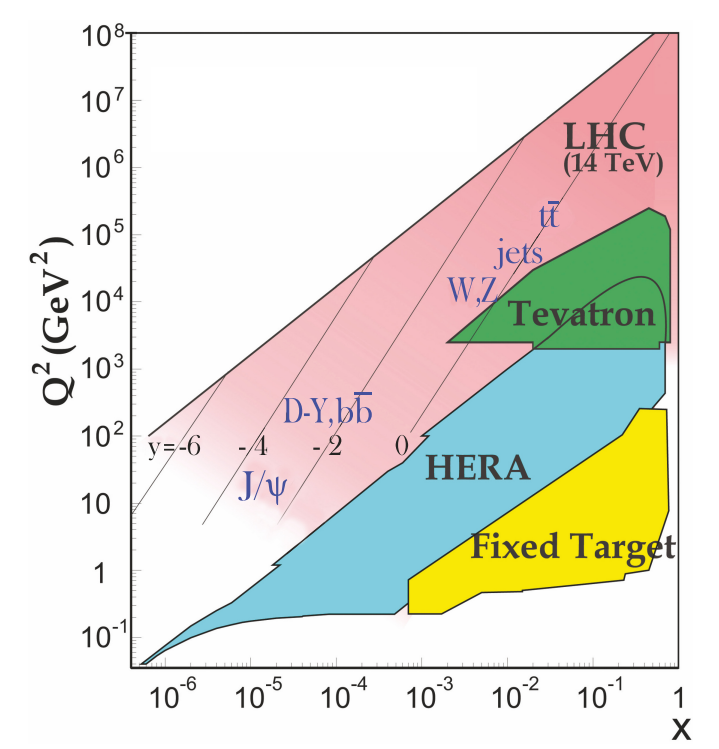
\includegraphics[width=0.8\linewidth]{images/NuProp/reald}
\caption{Кинематические области в $x$ и $Q^2$, исследованные в экспериментах с неподвижной мишенью и на коллайдерах. Рисунок из \cite{ParticleDataGroup:2024cfk}.}
\label{fig:xQ2_PDG}
\end{figure}

\subsection{Вклад экспериментально недоступной области}
Для иллюстрации, на рис.~\ref{fig:diff_xsec_100PeV} приведено дважды дифференциальное нормированное сечение
\[
\frac{1}{\sigma(E_\nu)}\frac{d^2\sigma(E_\nu,x,Q^2)}{dx\,dQ^2}
\] 
как функция переменных $x$ и $Q^2$ при энергии нейтрино $E_{\nu} = 100$ ПэВ. $\sigma(E_\nu)$ - полное сечение глубоконеупругого взаимодействия нейтрино с нуклоном при фиксированной энергии нейтрино. 

На рисунке также приведена заштрихованная область, качественно отражающая экспериментально исследованную область, представленную на рис.~\ref{fig:xQ2_PDG}.
\begin{figure}[!h]
\centering
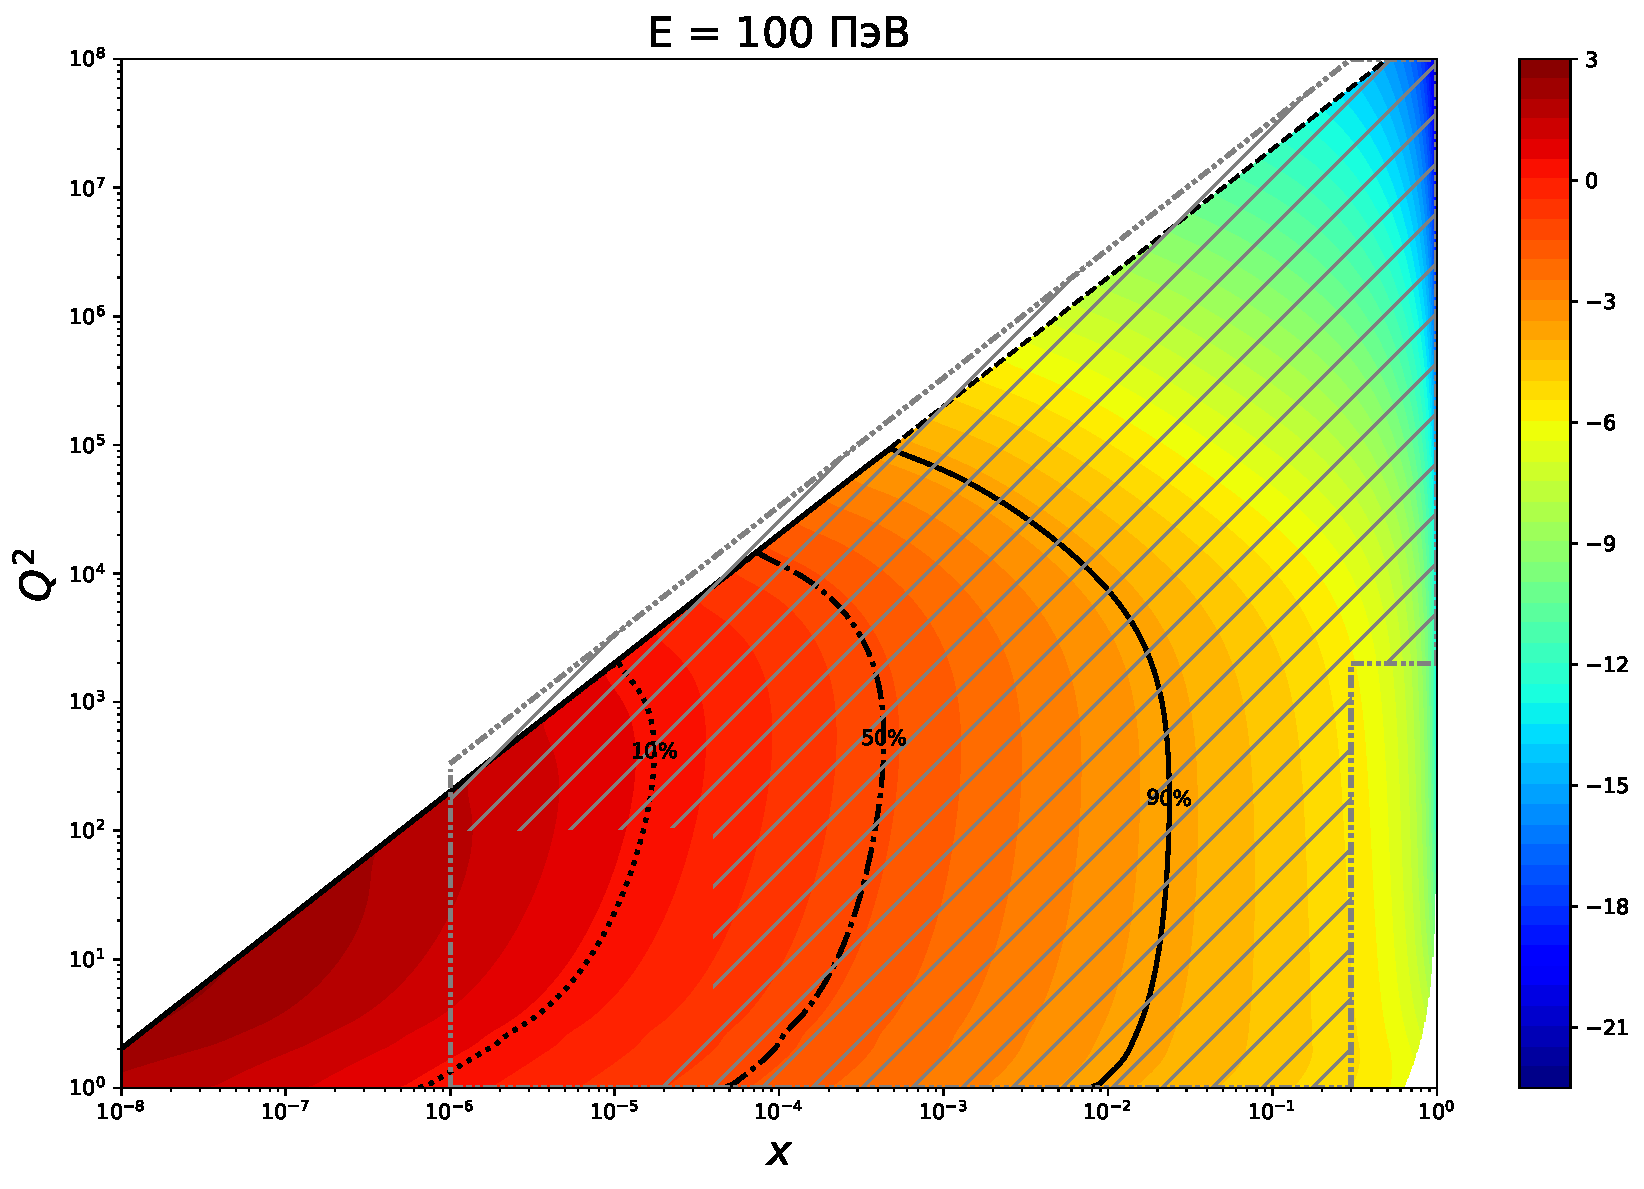
\includegraphics[width=0.8\linewidth]{images/NuProp/cdfxq2_cc_proton_CT18ZNNLO_14_100000000.pdf}
\caption{Дважды дифференциальное ормированное сечение $\frac{1}{\sigma(E_\nu)}\frac{d^2\sigma(E_\nu,x,Q^2)}{dx\,dQ^2}$ как функция $x$ и $Q^2$ для энергии нейтрино $E_{\nu} = 100$ ПэВ. Использованы партонные распределения CTEQ15\cite{ncteq15}.}
\label{fig:diff_xsec_100PeV}
\end{figure}

В области $x\lesssim 10^{-6}$, где экспериметальные данные отсутствуют, $\frac{1}{\sigma(E_\nu)}\frac{d^2\sigma(E_\nu,x,Q^2)}{dx\,dQ^2}$ максимально.  Пунктирные линии в пространстве $x,Q^2$ на рисунках указывают области, где сечения насыщаются до определенного уровня: $10\%$, $50\%$, $90\%$. Можно сделать заключение, что вклад области $x\lesssim 10^{-6}$ порядка $5\%$. В приложении~\ref{sec:examples_extrapolated_region} приведены еще два примера аналогичных распределений для энергий нейтрино 1 ТэВ и 1 ПэВ. 

Более простой способ оценки заключается в том, чтобы пренебречь сложной зависимостью двумерной области $x,Q^2$, в которой существуют экспериментальные измерения, а сосредоточиться только на главной в данном контексте переменной - $x$ Бьёркена. Определим отношение: 
\begin{equation}
\frac{1}{\sigma(E_\nu)}\int\limits_{x}^1\,\frac{d\sigma(E_\nu,x')}{dx'}dx',
\label{eq:CDF_x}
\end{equation}
где 
\[
\frac{d\sigma(E_\nu,x)}{dx} = \int\limits_0^{1}dy\,\frac{d^2\sigma(E_\nu,x,y)}{dx\,dy}.
\]
На рис.~\ref{fig:CDF_x} приведена функция~\eqref{eq:CDF_x} в зависимости от $x$ и $Q^2$ для треё значений энергии нейтрино $E_{\nu}= $ 1 ТэВ, 1 ПэВ, 100 ПэВ.
\begin{figure}[!h]
\centering
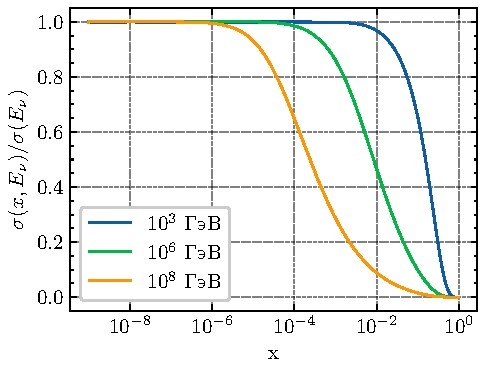
\includegraphics[width=0.8\linewidth]{images/NuProp/cdfxy_plot_CT18ZNNLO_14.pdf}
\caption{Функция $\int\limits_{x}^1\,\frac{1}{\sigma(E_\nu)}\frac{d\sigma(E_\nu,x')}{dx'}dx'$ в зависимости от $x$ и $Q^2$ для треё значений энергии нейтрино $E_{\nu}= $ 1 ТэВ, 1 ПэВ, 100 ПэВ. Использованы партонные распределения CTEQ15\cite{ncteq15}.}
\label{fig:CDF_x}
\end{figure}


\subsection{Полное сечение и его вариация от параметризации}
Из первых принципов довольно сложно оценить вклад неисследованной области в величину полного сечения. Косвенный метод - использовать вариацию в полном сечении при использование различных теоретических параметризаций.  На рис.~\ref{fig:xsec_total} показана зависимость полного сечения взаимодействия мюонного нейтрино на нуклоне от энергии для различных партонных распределений. Также, приведена вариация полного сечения, связанная с использовании разных наборов партонных распределений. Можно сделать вывод о том, что оценка на уровне $5\%$ вариации отвечает наблюдению из предыдущего раздела.

\begin{figure}[!h]
\centering
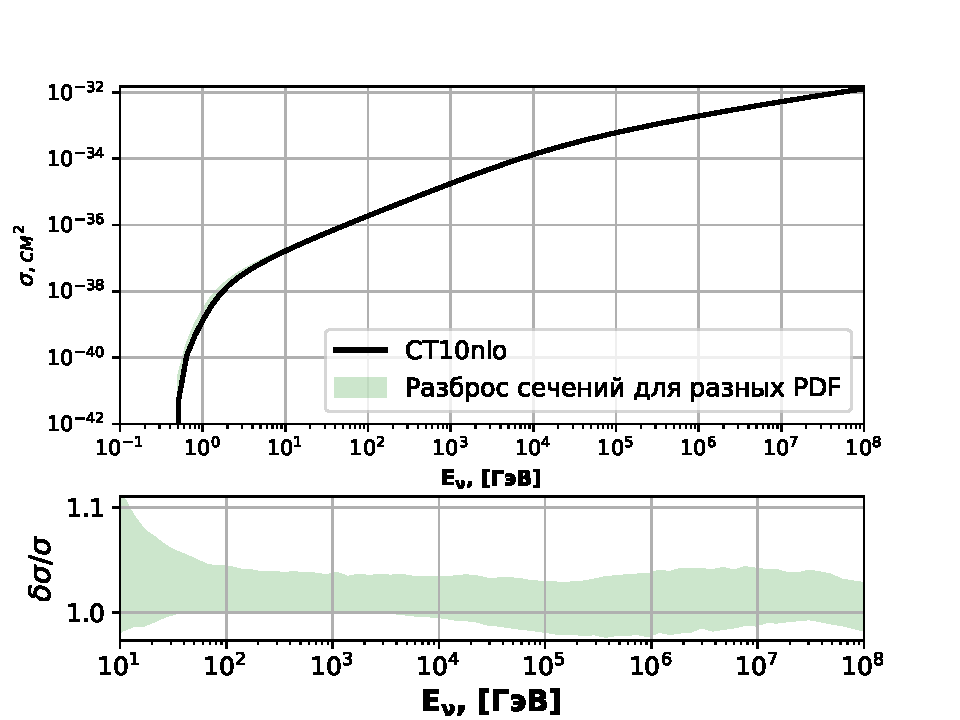
\includegraphics[width=\linewidth]{images/NuProp/xs_vs_enu.pdf}
\caption{Полные сечения взаимодействия мюонного нейтрино на нуклоне в зависимости от энергии $E_\nu$ для партонных распределений \texttt{CT10nlo}. Полоса отвечает вариации полного сечения при использовании других наборов партонных распределений (\texttt{CT18ZNNLO}, \texttt{nCTEQ15}, \texttt{TUJU19\_nlo}).} 
\label{fig:xsec_total}
\end{figure}
